\documentclass[11pt]{article}

\usepackage[utf8]{inputenc}
\usepackage[T1]{fontenc}
\usepackage{lmodern}
\usepackage[margin=1in]{geometry}
\usepackage{amsmath}
\usepackage{booktabs}
\usepackage{graphicx}
\usepackage{caption}
\usepackage{enumitem}
\usepackage[hidelinks]{hyperref}
\usepackage{xcolor}

\graphicspath{{../figures/}}

\newcommand{\code}[1]{\texttt{#1}}

\title{When impurity importance misleads:\\
interactions, non-linearity, and feature scale}
\author{Christian Theil Have}
\date{Original note: 17 May 2022. Validated and rewritten: July 2026.}

\begin{document}
\maketitle

\begin{abstract}
Mean-decrease-in-impurity (MDI) variable importance is the default, cheapest way
to read a random forest, and it is routinely compared, informally, to the
coefficients of a linear model. This paper examines when that comparison breaks
down. Through five controlled experiments (all reproduced with \code{ranger}) we
show that impurity importance (i) orders linear effects correctly but magnifies
them super-linearly, (ii) charges interaction effects to the interacting
variables, even when those variables have no marginal effect at all, and
(iii)~--- the central result --- \emph{cannot distinguish a genuinely non-linear
effect from a linear effect acting on a skewed feature}. The two produce
identical importances. The root cause is that regression trees split on variance
reduction, and variance is not scale-invariant. We argue that impurity importance
should be read as a detector of \emph{structure worth investigating}, not as an
effect-size estimate, and that partial-dependence plots recover the distinction
that importance discards. A screen of the ranger-citing literature
(Section~\ref{sec:prevalence}) finds the pitfall in roughly 10\% of
importance-using papers, including foundational, heavily-cited work.
\end{abstract}

\section{Background}

For a random forest, the impurity importance of a feature is the total decrease
in node impurity attributable to splits on that feature, summed over all splits
and all trees. For classification the impurity is Gini; for regression there is
no class label at a node, so \code{ranger} (and most implementations) use
\textbf{response variance} as the impurity proxy --- a split is scored by how
much it reduces the sum of within-child variances. This substitution is the
source of every effect studied here.

Impurity importance is known to be biased: it favours continuous and
high-cardinality features and inflates the importance of correlated predictors
(Strobl et al.\ 2007; Nembrini et al.\ 2018, \emph{The revival of the Gini
importance?}, which introduces the bias-corrected ``actual impurity reduction'',
AIR, exposed by \code{ranger} as \code{importance = "impurity\_corrected"}). The
question here is narrower and more practical: \textbf{if I line up impurity
importances next to OLS coefficients, when will I be misled?}

All experiments use \code{ranger} 0.18.0; the driver is
\code{analysis/validate.R} and figures come from \code{analysis/figures.R}.
Unless noted, importances are the plain \code{impurity} measure (the one the
definition above describes); Section~\ref{sec:linear} compares it against
\code{impurity\_corrected}.

\section{Linear effects: right order, wrong magnitude}
\label{sec:linear}

Data: $y = a + 2b + 4c$, with $a,b,c \sim U(0,1)$, $n = 1000$. OOB
$R^2 = 0.98$. Impurity importance ranks the features in the correct order, but
the \emph{ratios} are distorted:

\begin{center}
\begin{tabular}{rccc}
\toprule
feature & OLS coef & impurity vip (ratio) & impurity\_corrected (ratio) \\
\midrule
a & 1 & 1.00 & 1.00 \\
b & 2 & 2.32 & 5.31 \\
c & 4 & 7.79 & 23.1 \\
\bottomrule
\end{tabular}
\end{center}

A coefficient ratio of $1:2:4$ becomes an importance ratio of $1:2.3:7.8$. The
magnification is \textbf{super-linear}. Extending to
$y = a + 2b + 3c + \dots + 11k$ (11 features, coefficients $1\ldots11$) and
regressing importance on effect size, a linear fit gives $R^2 = 0.91$ while a
quadratic fit gives $R^2 = 0.97$ (Fig.~\ref{fig:superlinear}). Importance scales
roughly with the \emph{square} of the coefficient, because a feature with a
larger coefficient contributes more variance per split \emph{and} is chosen for
more splits.

Note the bias correction makes this \textbf{worse}, not better:
\code{impurity\_corrected} de-biases null (no-effect) features but does not
restore scale-invariance among real effects --- its ratios ($1:5.3:23$) are more
extreme than plain impurity's.

\begin{figure}[htb]
\centering
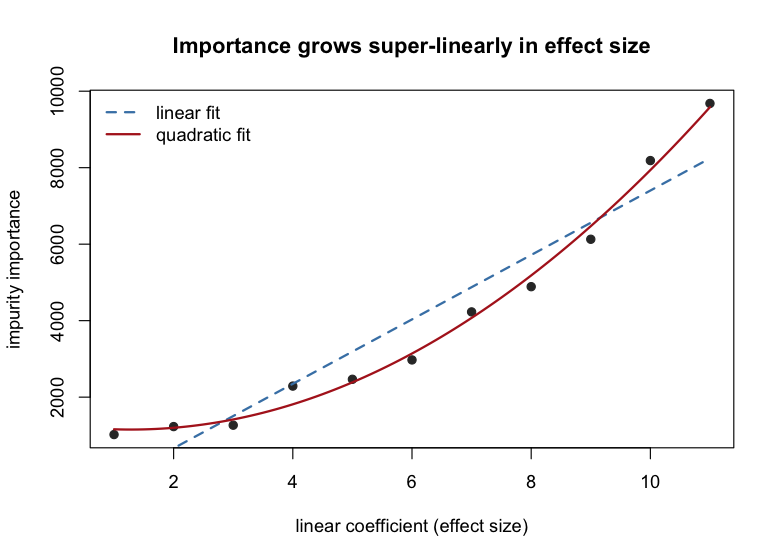
\includegraphics[width=0.72\textwidth]{fig1_superlinear.png}
\caption{Impurity importance vs.\ linear coefficient. The quadratic fit (red)
dominates the linear fit (blue dashed).}
\label{fig:superlinear}
\end{figure}

\paragraph{Takeaway.} Importance answers ``which feature matters more'' reliably
for linear effects, but ``how much more'' is not comparable to a coefficient.

\section{Interactions are charged to the interacting variables}
\label{sec:interactions}

Data: a pure parity interaction with no marginal effects,
\[
  y = c/10 + \big((a + b) \bmod 2\big), \qquad a,b,c \in \{0,1\}, \quad n = 10000.
\]
$a$ and $b$ individually carry no information about $y$; only their parity does.
$c$ has a small independent effect.

\begin{itemize}[leftmargin=1.4em]
\item \textbf{OLS} is blind: $R^2 = 0.01$, and the fitted coefficients for $a$
  and $b$ are exactly 0 (only $c$ survives, coef $\approx 0.10$). A standard
  $a{\times}b$ product term does not rescue it --- the interaction is non-linear
  (parity), not the bilinear form OLS interaction terms assume.
\item \textbf{Random forest} captures it: OOB $R^2 = 0.63$. And the impurity
  importance loads almost entirely on the interacting variables:
  $\mathrm{vip}(a) = 483$, $\mathrm{vip}(b) = 503$, $\mathrm{vip}(c) = 16$
  (Fig.~\ref{fig:interaction}). The interaction variables outrank the one
  variable with a genuine marginal effect by ${\sim}30\times$.
\end{itemize}

\begin{figure}[htb]
\centering
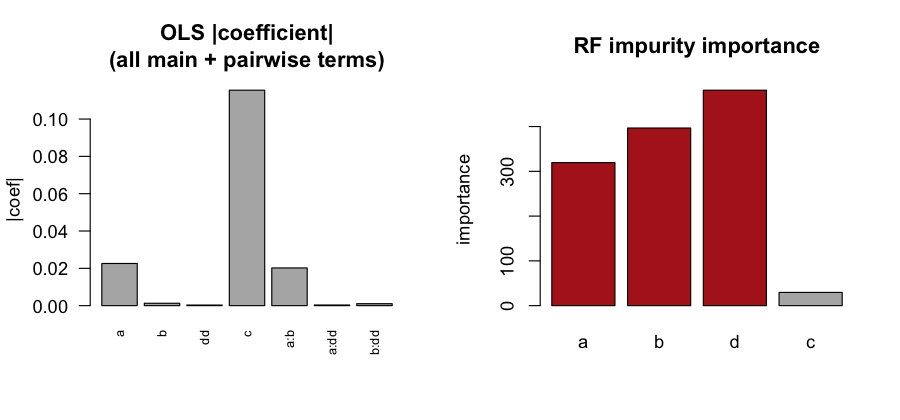
\includegraphics[width=0.85\textwidth]{fig2_interaction.png}
\caption{Same data, two views. OLS assigns $a,b$ zero coefficient; RF impurity
importance ranks them highest.}
\label{fig:interaction}
\end{figure}

\paragraph{Takeaway.} A high impurity importance does \textbf{not} imply a
detectable marginal effect. This is a feature, not a bug: importance surfaces
variables that matter only in combination --- precisely the ones a naive linear
model drops. But it means importance and coefficients measure different things.

\section{Why variance-splitting favours large-scale, non-linear structure}
\label{sec:variance}

Take a noise-free, sorted dataset and sweep every possible single split, scoring
each by the sum of within-child variances. For $y = x$, $y = x^2$, $y = x^3$
($x = 1\ldots1000$):

\begin{center}
\begin{tabular}{ccc}
\toprule
response & min split-variance & argmin index (of 1000) \\
\midrule
$x$   & $4.2 \times 10^{4}$  & 500 (centre) \\
$x^2$ & $4.3 \times 10^{10}$ & 697 \\
$x^3$ & $4.1 \times 10^{16}$ & 799 \\
\bottomrule
\end{tabular}
\end{center}

Two mechanisms compound:
\begin{enumerate}[leftmargin=1.6em]
\item \textbf{Scale.} The achievable variance reduction grows by orders of
  magnitude with the polynomial degree. Splits driven by high-order
  (large-range) structure dominate the split-selection criterion, and each such
  split books a larger impurity decrease.
\item \textbf{Imbalance.} For a linear response the best split is central; for
  higher orders the optimal split migrates toward the high-$y$ tail (index
  $500 \rightarrow 697 \rightarrow 799$). Unbalanced splits leave more structure
  in the large child, so \emph{more} splits are needed --- and every one of them
  is charged to the same feature.
\end{enumerate}

Variance is not scale-invariant, so whatever varies on the largest scale wins
twice.

\section{Non-linear effects (Section~\ref{sec:variance} confirmed on real forests)}
\label{sec:nonlinear}

Data: $y = a + b^2 + c^3$, features ${\sim}\,1+U(0,1)$, $n = 10000$. As predicted,
$\mathrm{vip}(a) < \mathrm{vip}(b) < \mathrm{vip}(c)$:
$1780 < 8168 < 39570$. Importance rises faster than the degree of the term. A
linear model still estimates non-zero coefficients here, but they are
uninterpretable --- the residuals are visibly non-normal, signalling the
misspecification.

\section{The central confound: non-linearity vs.\ feature scale are indistinguishable}
\label{sec:confound}

This is the result that should change how the measure is read. Construct data
with \textbf{exactly equal linear effects}, but skewed feature
\emph{distributions}:
\[
  a = 1 + U, \quad b = (1 + U)^2, \quad c = (1 + U)^3, \quad y = a + b + c,
  \quad n = 10000.
\]
Every feature enters $y$ with coefficient 1. OLS confirms it: fitted coefficients
are $1.00, 1.00, 1.00$. Each unit increase in $a$, $b$, or $c$ moves $y$ by one
unit --- there is nothing non-linear about the \emph{effects}.

Yet the random forest reports importances of \textbf{1780 / 8168 / 39570} --- a
$1:4.6:22$ spread. These are not merely unequal; they are \textbf{numerically
identical} to the non-linear-effects model of Section~\ref{sec:nonlinear}
(Fig.~\ref{fig:confound}). The forest cannot tell the two generating processes
apart, because both present the same \emph{marginal variance structure} to the
splitting criterion: a feature whose values are spread over a cubic range
delivers the same variance-reduction opportunities whether the cubic lives in the
effect ($c^3$) or in the feature ($c \sim U^3$).

\begin{figure}[htb]
\centering
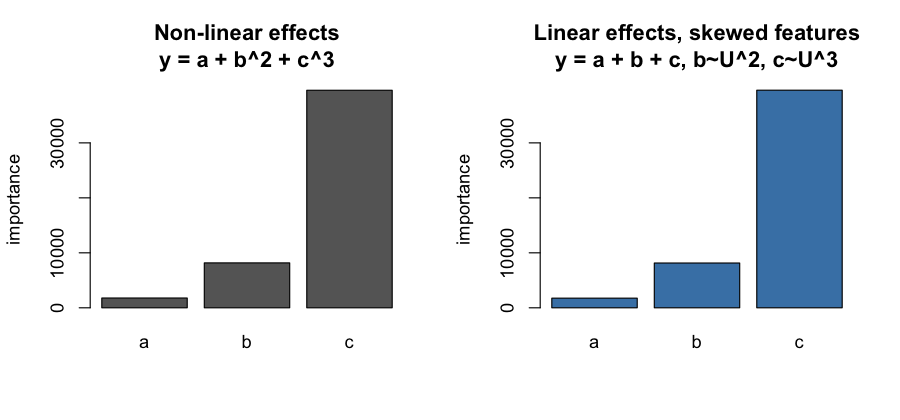
\includegraphics[width=0.85\textwidth]{fig3_confound.png}
\caption{Identical importances from two different worlds. Left: genuinely
non-linear effects. Right: linear effects on skewed features. Impurity importance
cannot distinguish them.}
\label{fig:confound}
\end{figure}

A split-variance sweep on the skewed-feature data confirms the mechanism: median
achievable split-variance is lowest for $c$ (4.4) and highest for $a$ (9.8), so
$c$ is split earlier and more often --- matching the importance ranking, even
though $c$'s effect on $y$ is no larger than $a$'s.

\paragraph{Takeaway.} Impurity importance conflates \emph{effect non-linearity}
with \emph{feature skew}. A tall importance bar can mean ``this feature has a
strong/non-linear effect'' \textbf{or} merely ``this feature has a
wide/heavy-tailed distribution.'' The measure alone cannot say which.

\section{Practical guidance}

\begin{enumerate}[leftmargin=1.6em]
\item \textbf{Read impurity importance ordinally, and only among comparable
  features.} Treat it as a ranked shortlist of variables worth investigating, not
  as an effect size. Never place its magnitudes alongside OLS coefficients as if
  they were the same currency.
\item \textbf{A high bar is a prompt, not a conclusion.} It may reflect a marginal
  effect, an interaction (Section~\ref{sec:interactions}), a non-linear effect
  (Section~\ref{sec:nonlinear}), or nothing but a skewed feature distribution
  (Section~\ref{sec:confound}).
\item \textbf{Disambiguate with partial-dependence plots.} PDPs recover exactly
  what importance discards: in Section~\ref{sec:confound} the skewed-feature
  model's PDPs are straight lines while the non-linear model's curve --- same
  importances, different shapes. PDPs also expose the checkerboard signature of
  the Section~\ref{sec:interactions} interaction that per-feature importance
  flattens. Curvature in a PDP is a concrete cue to add a polynomial or
  interaction term back into an interpretable model.
\item \textbf{\code{impurity\_corrected} fixes a different problem.} It removes
  the bias toward null / high-cardinality features (use it --- it is the right
  default), but it does not make importances scale-comparable across real
  effects; if anything it widens the spread (Section~\ref{sec:linear}).
\item \textbf{If you know the structure is linear, use the linear model.} Random
  forests buy you interaction- and non-linearity-detection; when there is nothing
  to detect, OLS is both more accurate and directly interpretable.
\end{enumerate}

\section{How often does this happen in practice?}
\label{sec:prevalence}

To gauge whether the pitfall is real in the wild, we audited the published
literature that uses the tool most associated with these importances --- the
\code{ranger} R package. Full method and numbers are in
\code{analysis/results.md}; the short version:

\begin{itemize}[leftmargin=1.4em]
\item \textbf{Corpus.} All 3{,}189 works citing ranger (OpenAlex
  \code{W2157395790}), fetched via the OpenAlex and Europe PMC APIs; 773 have
  open-access full text. A versioned regex filter (\code{analysis/fingerprint.py})
  kept the 524 that mention variable/feature/impurity importance (dropping papers
  that cite ranger only for speed or prediction); 544 were screened in total.
\item \textbf{Stage 1 --- screening (Claude Haiku 4.5, low effort).} One agent per
  paper read the full text and emitted a structured record. It was told the
  specific bias under audit --- \emph{impurity importance corrupts the magnitude
  and ranking of an effect, not the yes/no verdict of whether a variable is used;
  a significant importance p-value (Altmann/Janitza/Boruta) tests only that
  importance $\neq 0$, which is robust} --- and instructed to set the flag
  (\code{p\_affected} $\wedge$ \code{central\_to\_conclusions}) true only when a
  paper leans on the \textbf{magnitude or ranking} of impurity importance for a
  central conclusion \textbf{without} adequate corroboration, where adequate
  corroboration = permutation importance, SHAP, PDP/ALE, conditional importance,
  or held-out validation of the \emph{selected feature set} (overall model
  accuracy does not count). Every judgement had to quote supporting passages.
  125 papers were flagged.
\item \textbf{Stage 2 --- adjudication (Claude Sonnet 5, high effort).} A second,
  independent agent re-read each flagged paper under an explicitly
  \textbf{adversarial} instruction: \emph{your job is to refute this flag}. It
  confirmed only when all three held --- the paper genuinely uses impurity (not
  only permutation/SHAP) importance, the ranking is central to a conclusion, and
  the ranking is not adequately corroborated --- and was told to reach its own
  verdict rather than defer to stage 1. It returned
  \code{confirmed}/\code{refuted}/\code{uncertain} with reasons.
\item \textbf{Result: 55 confirmed, 65 refuted, 5 uncertain} --- the adversarial
  pass overturned ${\sim}56\%$ of the screening flags (so stage-1 precision
  ${\approx}44\%$). The 55 confirmed are \textbf{${\sim}10\%$ of the
  importance-using full-text papers} --- roughly 7\% of all full-text
  ranger-citing work. The full prompts, per-paper records, and verdicts are in
  \code{analysis/} (\code{extract\_broad\_workflow.js},
  \code{adjudicate\_workflow.js}, \code{extraction/}, \code{adjudication/}).
\item \textbf{The exposure is not in the careful literature.} 86\% of flagged
  papers use no significance machinery at all (no \code{importance\_pvalues},
  Altmann, Janitza, or Boruta) --- they simply rank features by impurity
  importance. Papers that \emph{do} use those methods, and the rising share
  (${\sim}0\% \rightarrow {\sim}70\%$ over 2016--2026) that pair importance with
  SHAP/permutation/PDP, are markedly less exposed.
\item \textbf{It reaches high-impact work.} The single most-cited confirmed case
  is \textbf{SoilGrids250m} (Hengl et al., \emph{PLoS ONE} 2017; 4{,}684
  citations), a global soil-property product whose covariate ranking is read
  straight off ranger/xgboost built-in importance. Tellingly, the authors note
  lithology visibly drives predictions yet falls outside the top-15 importance
  list --- the exact signature of Sections~\ref{sec:variance}
  and~\ref{sec:confound}, a low-cardinality categorical under-weighted against
  fine-grained continuous covariates.
\end{itemize}

Caveats: these are LLM screening judgements, not audits of each study's data ---
a confirmed flag means a conclusion \emph{could} have been distorted and was not
cross-checked, not that it is wrong. Predictive accuracy, validated separately,
is unaffected. Proving a specific ranking is altered requires re-running the
study's model with an unbiased measure.

\section{Conclusion}

Impurity importance is a variance-reduction accounting, and variance is neither
scale-invariant nor able to separate an effect's shape from a feature's
distribution. Consequently it magnifies effect sizes super-linearly, attributes
interaction effects to marginally-null variables, and --- most importantly ---
returns identical scores for genuinely non-linear effects and for linear effects
on skewed features. Every claim in the 2022 note reproduces cleanly, and a
literature audit (Section~\ref{sec:prevalence}) confirms the pitfall is not merely
theoretical: ${\sim}10\%$ of importance-using ranger papers --- including
foundational, heavily-cited products --- lean on impurity rankings without the
corroboration that would catch it. Used as a \emph{screening} tool and paired with
partial-dependence plots to interrogate the shortlist, impurity importance is
valuable; read as a substitute for effect sizes, it will mislead.

\section*{Reproducing}

\begin{verbatim}
brew install r
R_LIBS_USER=./.rlib Rscript -e 'install.packages(c("ranger","tibble","pdp"),
                                  repos="https://cloud.r-project.org")'
R_LIBS_USER=./.rlib Rscript analysis/validate.R  # prints every number cited above
R_LIBS_USER=./.rlib Rscript analysis/figures.R   # regenerates figures/
\end{verbatim}

\begin{thebibliography}{9}
\bibitem{nembrini2018} Nembrini, K\"onig, Wright (2018). \emph{The revival of the
  Gini importance?} Bioinformatics 34(21).
  \url{https://www.ncbi.nlm.nih.gov/pmc/articles/PMC6198850/}
\bibitem{strobl2007} Strobl, Boulesteix, Zeileis, Hothorn (2007). \emph{Bias in
  random forest variable importance measures.} BMC Bioinformatics.
\bibitem{scheidel2018} Scheidel (2018). \emph{Be aware of bias in RF variable
  importance metrics.}
\bibitem{lee2017} Lee (2017). \emph{Feature Importance Measures for Tree Models
  --- Part I.}
\bibitem{soilgrids2017} Hengl et al.\ (2017). \emph{SoilGrids250m: Global gridded
  soil information based on machine learning.} PLoS ONE 12(2): e0169748.
\end{thebibliography}

\end{document}
